\chapter{Current peak transducer}
\section{Theory and related work} \label{sec:literature_current_peak_transducer}
The design for the current peak transducer consisted of a current sense resistor in series with the load, a non inverting operational amplifier gain stage, and a precision rectifier implemented as in Section \ref{sec:design_voltage_peak_transducer}. A current sense resistor is a resistor placed in series with a load to allow current to be measured, the voltage across the resistor will be directly proportional to the current being measured. A non inverting amplifier is an operational amplifier configuration where the input voltage signal is connected to the non-inverting input to the operational amplifier. The feedback control consists of a resistor divider network that connects the output to the inverting input, this resistor divider network sets the gain of the amplifier, produces a good stability and has a high input impedance \ref{yourmom}. 
%https://www.electronics-tutorials.ws/opamp/opamp_3.html

\section{Design} \label{sec:design_current_peak_transducer}
The first part of this design included a sense resistor which was added in series with the load to turn a current measurement into a voltage measurement, this voltage measurement was then amplified to a suitable voltage level usable by the peak transducer. For the purpose of this design a $\SI{30}{\milli \Omega}$ sense resistor was chosen to ensure a reasonable trade off between power losses in the system and the measured voltage level over the sense resistor. It was found that a smaller sense resistor would by Ohm's law have a smaller voltage drop over it, and this in return would require a larger voltage gain stage, which was not desirable as such a large gain would require a very large feedback resistor, with a very large deviation from its given resistance. It was chosen that the current peak transducer would be able to measure a maximum current of \SI{350}{\milli A}, this corresponded to a sense voltage of \SI{10.5}{\milli V}.\newline
The Arduino's maximum pin voltage was given as \SI{5}{\volt}, and to ensure a maximum resolution for the \SI{350}{\milli A} measurement range, the \SI{10.5}{\milli V} maximum sense voltage had to be amplified using an operational amplifier. This operational amplifier configuration was chosen as a differential mode non-inverting amplifier utilizing only the SI{5}{\volt} and rail as its power supply. It was found that the maximum input to any of the operational amplifiers pins was not to exceed \SI{5}{\volt} or \SI{-0.3}{\volt} \ref{yourmom}.
The desired gain, and ratio between input resistor $R_1$, and feedback resistor $R_2$ was calculated by using Equation \ref{eq:opampgain}. Here $R_1$ was chosen as $\SI{1}{\kilo \Omega}$, and given this $R_2$ was found to be $\SI{470}{\kilo \Omega}$.\newline
\begin{equation}
   \frac{V_{out}}{V_{in}}=1+\frac{R_2}{R_1} 
   \label{eq:opampgain}
\end{equation}
Given that the sense voltage was now amplified to a suitable range between 0 and \SI{5}{\volt} the same design procedure as Section \ref{sec:design_voltage_peak_transducer} could be applied to measure the amplitude of the peak of the sinusoidal input. A ripple voltage of no more than \SI{5}{\milli \volt} was chosen and from this the output capacitor to the peak detector was calculated in exactly the same way as in Section \ref{sec:design_voltage_peak_transducer} using Equation \ref{eq:ripplevoltage}, the desired capacitor value was found as $\SI{20}{\micro F}$. To minimise the effect of noise on the output of the transducer the smoothing capacitor at the output was chosen as two \SI{10}{\micro F} low ESR capacitors placed in parallel. Decoupling capacitors were also placed at the positive rail of the TLC2272 to keep the effects of the rail voltage noise from the power supply to a minimum on the output.
Given the specification of a maximum load current of \SI{350}{\milli A} corresponding to a voltage of $\SI{5}{VAC}$ and the Arduino having a range of $4095$ bits, it can be calculated that the resolution of the ADC would be $\SI{85.47}{\micro A}$ per bit.
\begin{figure}[h!]
    \centering
    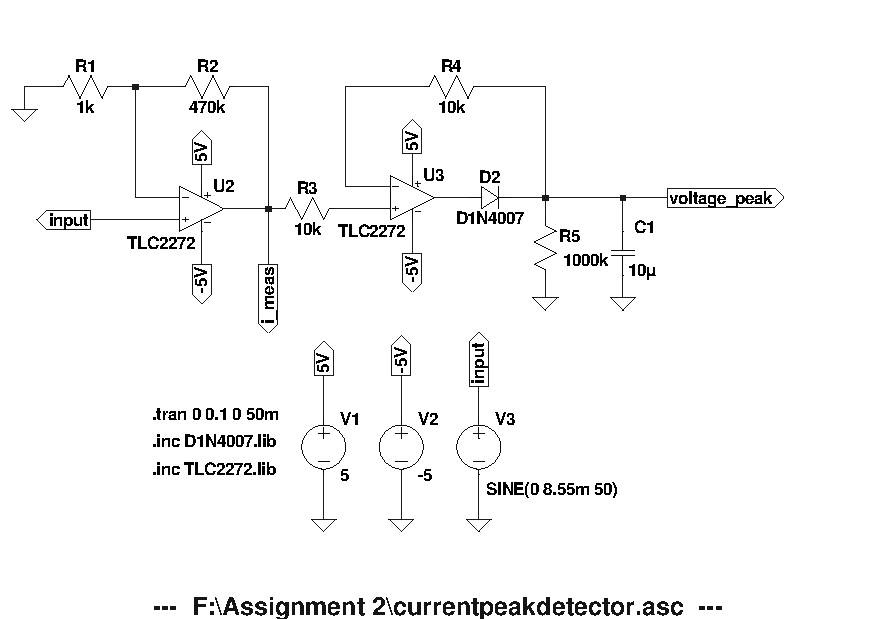
\includegraphics[width = 0.57\linewidth]{Figures/currentpeakdetector.pdf}
        \caption{Current Peak Transducer Diagram}
    \label{fig:currentpeakdetector.pdf}
\end{figure}

\section{Simulation} \label{sec:simulation_current_peak_transducer}
To confirm that the current peak transducer was designed correctly the designed circuit was supplied with a nominal input voltage of \SI{3}{\milli \volt}, this corresponded to a \SI{100}{\milli A} current through the sense resistor, this output can be seen in Figure \ref{subfig:currenttransducer100maripple}. From the output plot we can see that the ripple voltage was simulated to be \SI{9.2}{\milli \volt}, this was slightly higher than what was designed for in the design section, however for this purpose of this design the ripple voltage is acceptable as it does not interfere with the accuracy requirements of the current peak transducer measurement.\vspace{4mm} \newline 
To ensure that the current peak transducer responded to a \SI{10}{\milli A} change in input, for inputs over \SI{100}{\milli A}, within 1 second a \SI{3}{\milli \volt} input was applied and decreased by \SI{300}{\micro \volt}, this change in input voltage corresponded to a decrease in load current by \SI{10}{\milli A}. The result of this simulation can be seen in Figure \ref{subfig:currenttransducerinputchange}, and from this graph we can see that the input responded to the change in input in exactly 1 second. 

\begin{figure}[h!]
 \centering
     \begin{subfigure}[]{0.45\textwidth}
        \centering
         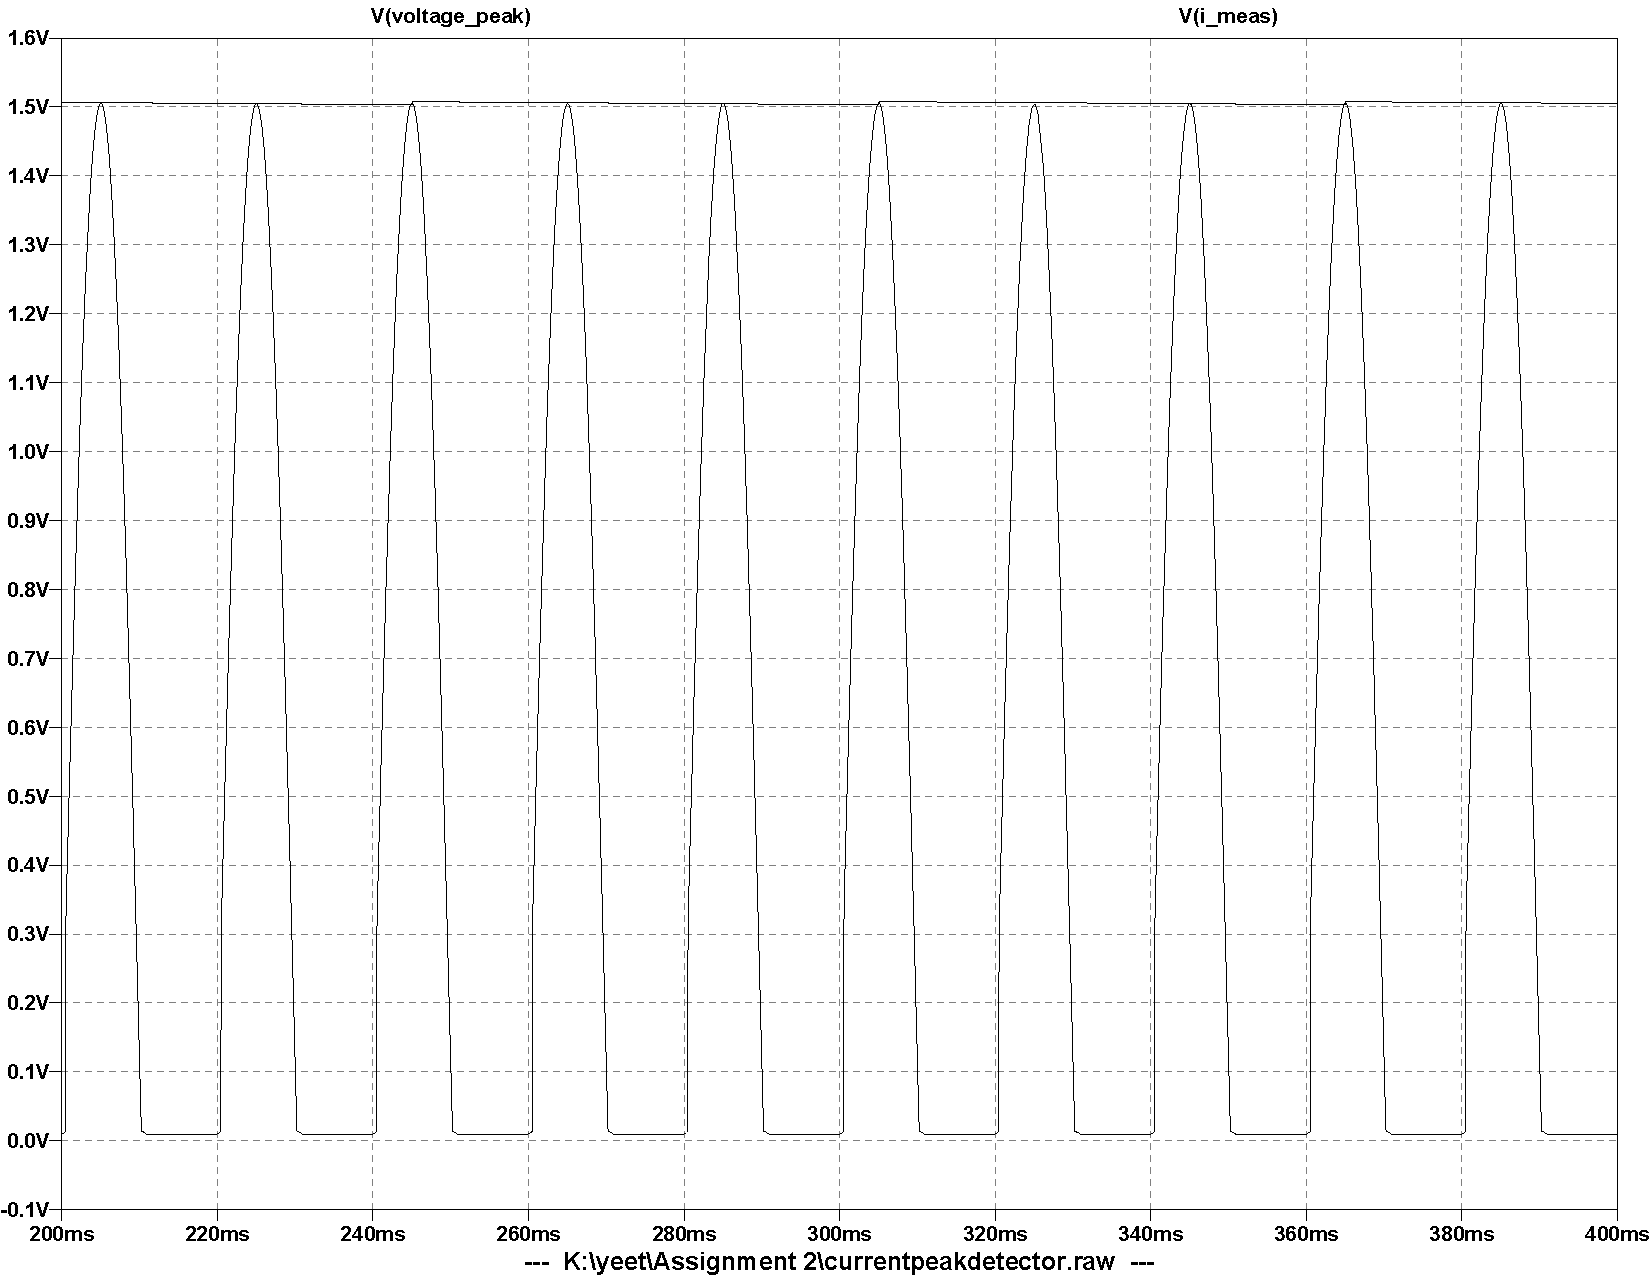
\includegraphics[width=1\linewidth]{./Figures/currentpeakdetectoroutputsim.pdf}
		    \caption{Peak detection of a amplified 100mA input} \label{subfig:currenttransducer100maripple}
     \end{subfigure}
      \begin{subfigure}[]{0.45\textwidth}
              \centering
  		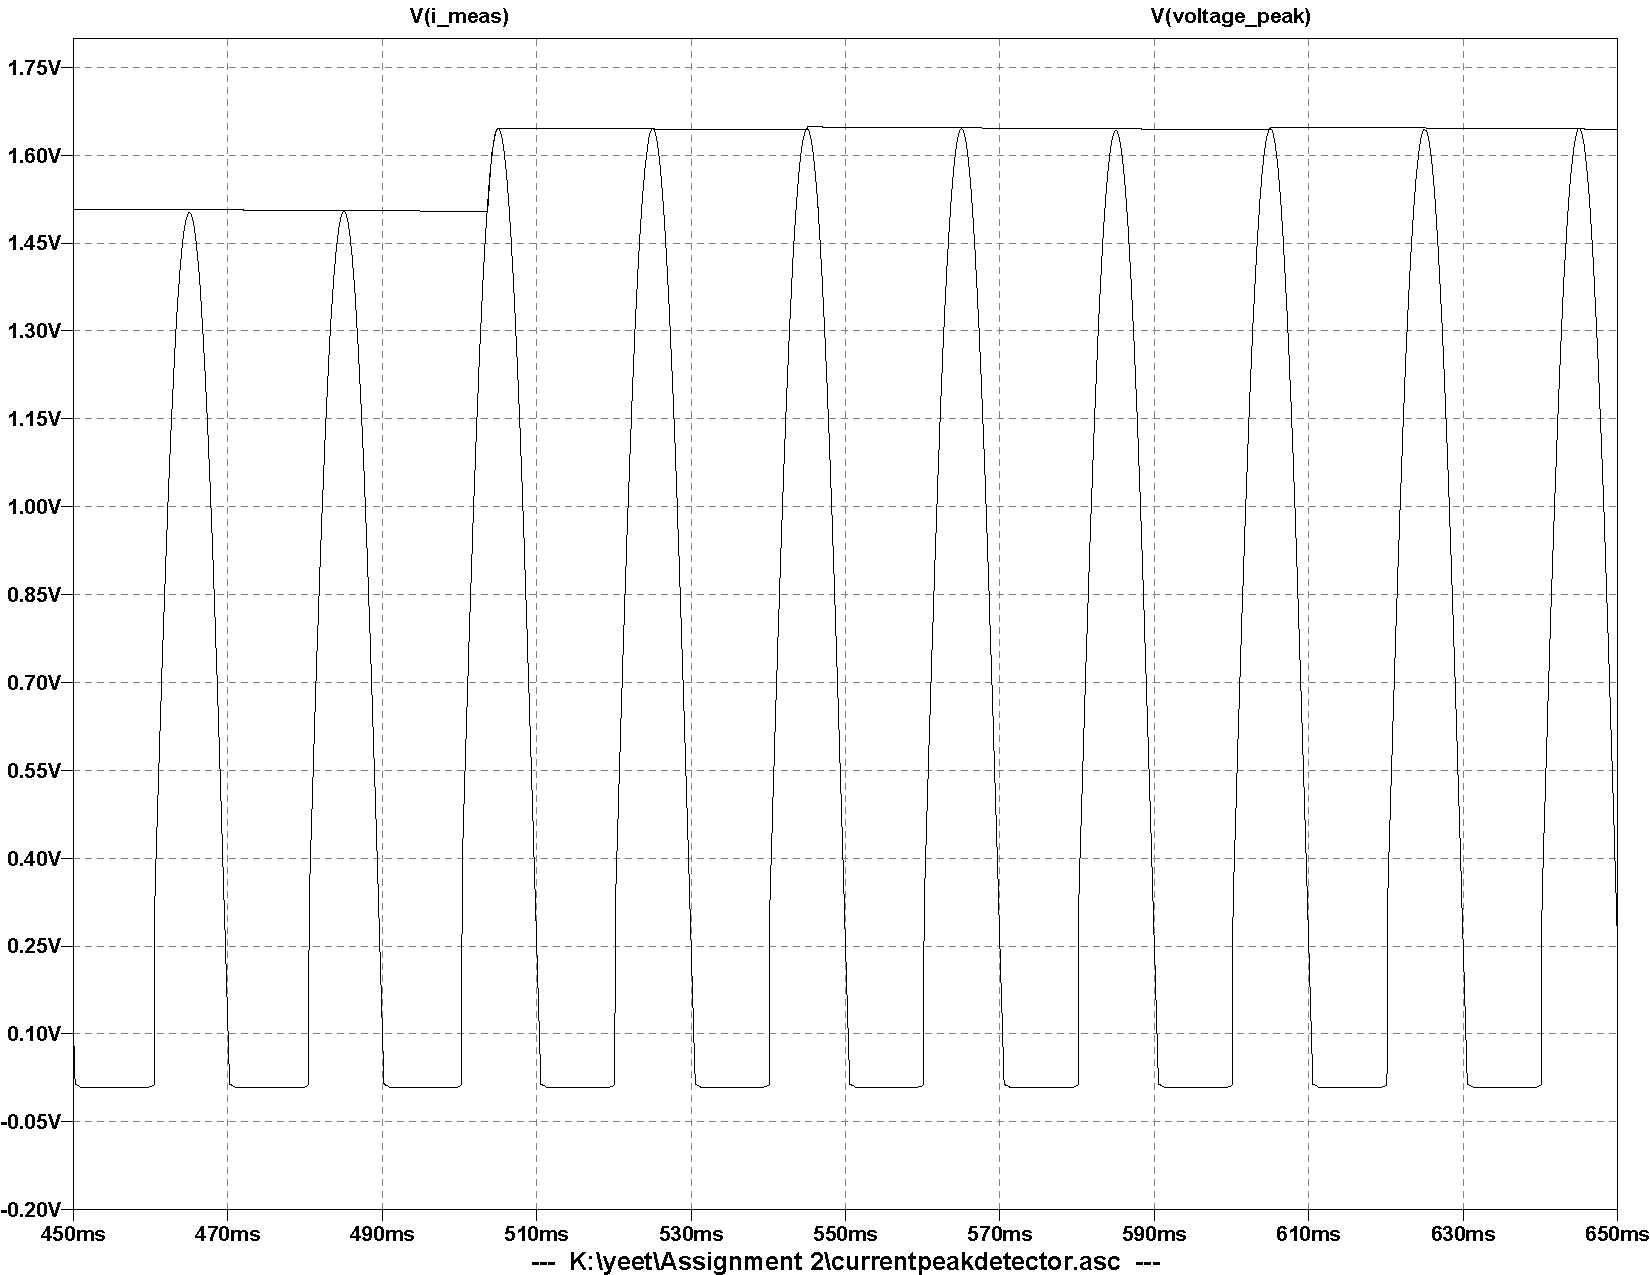
\includegraphics[width=1\linewidth]{./Figures/currentpeakdetectoroutputchange.pdf}
		    \caption{Response given \SI{10}{mA} change in \SI{100}{mA} input} \label{subfig:currenttransducerinputchange}
     \end{subfigure}
   \caption[Simulated results for the current transducer]{Output voltage ripple and response for the current transducer. (a) depicts output voltage ripple, (b) depicts response to change in input current. }
    \label{fig:simulation_results_box}
 \end{figure}


\section{Measurements} \label{sec:measurements_current_peak_transducer}
In order to test the accuracy and precision of the current peak transducer unit tests were performed using an oscilloscope and voltage divider. Since the oscilloscope could not output the small voltages required for the unit tests a voltage divider that divided the oscilloscope output down by a factor of 100 was required in order to obtain the sense voltages in the milli-Volt range. The input current was related to the output voltage by using Equation \ref{eq:currentcalc}. The gain of the operational amplifier gain stage was calculated to be $A_{v}=474.4$ using Equation \ref{eq:opampgain}, and the resistor values for this formula were measured using a multimeter.
\begin{align}
   V_{out}=R_{sense}I_{load}A_{v} \\
   V_{out}= 14.232I_{load} \nonumber
   \label{eq:currentcalc}
\end{align}
The second column in Table \ref{tab:currenttransducerunittests} shows the output as shown on the oscilloscope screen, and the third column shows the measurement found by measuring this output using an oscilloscope. This third column was the input to the voltage circuit, with the actual sense voltage being measured as these values divided by 100. All unit tests were found to be accurate within a maximum difference of only \SI{0.74}{\milli A}, confirming that the design met the requirements. \vspace{4mm} \newline 
The current peak transducer was then testing under real measurement conditions using various load resistors, these results are tabulated in Table \ref{tab:currenttransducerrealtests}, here it was found that all measurements except the no load test was within the \SI{1}{\milli A} design specification. This contradicts the result of the no load measurement difference shown in Table \ref{tab:currenttransducerunittests}, however this difference can be explained by the fact that the input to the operational amplifier was grounded by the signal generator for the unit test, and left floating for the real no load test. \vspace{4mm} \newline  
Figure \ref{subfig:currenttransducermidrange} shows the output of the current peak transducer given a load of  $\SI{1}{\kilo \Omega}$, from the oscilloscope measurements we can see that the difference between the signals is only $\SI{4}{\milli V}$, which by using Equation \ref{eq:currentcalc} is only out by $\SI{0.281}{\milli A}$. The signal quality of the transducer output is shown in Figure \ref{subfig:currenttransducermidrangenoise}, which has a peak to peak range of only $\SI{15.6}{\milli V}$. Due to the fact that the current peak transducer measurements were all within $\SI{1}{\milli A}$ of the actual measurement it was decided that no curve of best fit would be necessary to improve the output of this design.

\begin{table}[h]
        \centering
        \scriptsize
        \caption{Current transducer intermediate unit test results.}
             \begin{tabular}{C{2cm} C{2cm} C{2cm} C{2cm} C{2cm} C{2cm}}
           Emulated level & Signal generator & Signal generator & Analogue output & Deduced input & Difference \\
           ($mA_{peak}$)   & ($mV_{peak}$) & ($mV_{peak}$) & ($VDC$)         & ($mA_{peak}$) & ($mA_{peak}$) \\
           \hline
            0       & 0 & 0 & 0.004 & 0.281 & 0.28\\
            50      & 153.15 & 155.69 & 0.704 & 49.46   & 0.53\\
            100     & 309.12 & 311.32 & 1.416 & 99.49   & 0.51\\
            101     & 311.15 & 314.50 & 1.448 & 101.74  & 0.74\\
            102     & 316.60 & 317.61 & 1.456 & 102.30  & 0.30\\
            200     & 617.00 & 622.77 & 2.846 & 199.97  & 0.03\\
            285     & 879.50  & 887.20 & 4.064 & 285.55  & 0.55\\
          \hline
        \end{tabular}
     \label{tab:currenttransducerunittests}
\end{table}

\begin{table} [h]
        \centering
        \scriptsize
        \caption{Current transducer integrated test results.}
         \begin{tabular}{C{1.4cm} C{1.2cm} C{1.2cm} | C{1.8cm} C{1.8cm} C{2.2cm} C{2cm} C{1.8cm}}
           Measure- & Load $R_1$ & Load $R_2$ & Measured $V_R$ & Actual input & Analogue output & Deduced input & Difference\\
           ment & ($\Omega$) & ($\Omega$) & ($mV_{peak}$) & ($mV_{peak}$) & ($mV_{peak}$) & ($mA_{peak}$) & ($mA_{peak}$) \\
        \hline
            No load      & open & -   & 0      & 0      & 30.8  & 2.164   & 2.16\\
            Full load    & 100  & -   & 9.045       & 301.51 & 4.28  & 300.73  & 0.78\\
            Mid range    & 1k   & -   & 0.906       & 30.159 & 417.6 & 29.40 & 0.76 \\
            Mid + $\delta$    & 1k   & 24k  & 0.943 & 31.415 & 435.4 & 30.59 & 0.69 \\
          \hline
        \end{tabular}
     \label{tab:currenttransducerrealtests}
\end{table}

\begin{figure}[h]
 \centering
     \begin{subfigure}[]{0.45\textwidth}
        \centering
         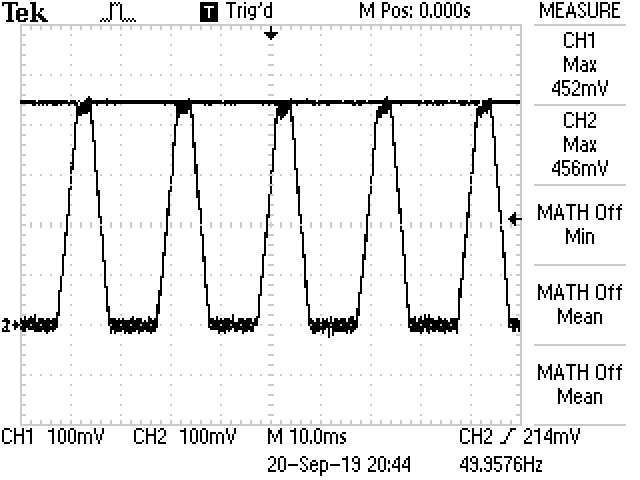
\includegraphics[width=1\linewidth]{./Figures/currenttransducermidrange.JPG}
		    \caption{Mid range measurement result} \label{subfig:currenttransducermidrange}
     \end{subfigure}
      \begin{subfigure}[]{0.45\textwidth}
              \centering
  		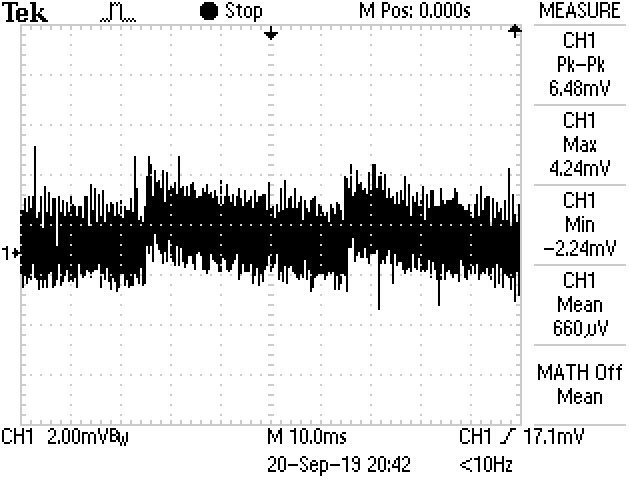
\includegraphics[width=1\linewidth]{./Figures/currenttransducernoise.JPG}
		    \caption{Noise response} \label{subfig:currenttransducermidrangenoise}
     \end{subfigure}
   \caption[Measured results for the current transducer]{Output voltage ripple and response for the current transducer. (a) depicts mid range output, (b) depicts noise response. }
    \label{fig:simulation_results_box}
 \end{figure}





